\section{Residual-Based Adaptive Refinement}
\label{sec:residual-adaptive}
\subsection{Motivation and controlled setup}
The reduced uniform energy rate, $p_E\simeq0.623$, and the absence of a measured advantage for the prescribed coordinate-line grading motivated a solution-driven extension. The hypothesis was recorded before the experiments in \texttt{logs/PRE\_ADAPTIVE\_HYPOTHESIS.md}. No advantage was assumed. The $8H$ domain, trace hole, material coefficient, homogeneous-Neumann far boundary, $P_1$ formulation and sparse direct solver were held fixed. No new all-air problem was solved, and the final M7 engineering values were not changed.

The historical M2 coordinates are left--right symmetric, but its identically oriented cell diagonals are not. To avoid confusing mesh-orientation asymmetry with adaptivity, the primary initial mesh uses a conforming, mirror-invariant subdivision of M1. All edge midpoints are inserted; each right triangle is divided into four nonobtuse triangles, giving exactly the M2 coordinates, $704$ elements and $404$ DOFs. We call this \emph{M1-S (M2-resolution)}, not the unchanged M2 triangulation. An eight-cycle M0-S companion path brackets the $0.40$ and $0.30$ error targets, since the primary initial error is already below $0.30$.

An earlier diagonal-only symmetry completion was rejected: its very coarse M0 companion produced minimum potentials down to about $-0.030$ V. All its points and timings remain in a separate failed-attempt directory and are excluded from the conclusions. The correction was made to satisfy potential bounds, not to optimise efficiency; the indicator and marking parameter were unchanged.

\subsection{Flux-jump indicator and marking}
For $f=0$, constant elementwise $\epsilon$ and affine $\phi_h|_K$, the interior volume residual vanishes. For an interior edge, choose one unit normal $n_e$ and define
\[
J_e=(\epsilon\nabla\phi_h|_{K^+}-\epsilon\nabla\phi_h|_{K^-})\cdot n_e.
\]
The same normal is used on both sides, including material-interface edges. With $h_e$ equal to edge length, the implemented indicator is
\begin{equation}
\eta_K^2=\frac12\sum_{e\subset\partial K\cap\mathcal E_{\rm int}}
h_e\|J_e\|_{L^2(e)}^2+
\sum_{e\subset\partial K\cap\Gamma_{\rm far}}
h_e\|\epsilon\nabla\phi_h\cdot n\|_{L^2(e)}^2,
\qquad \eta=\left(\sum_K\eta_K^2\right)^{1/2}.
\end{equation}
Since these traces are constant, each term is evaluated exactly as $h_e^2J_e^2$ (or its boundary counterpart). Trace and ground Dirichlet edges contribute no natural-boundary residual. This is a \emph{residual-based refinement indicator}, not a guaranteed error bound.

At every step, deterministic D\"orfler marking chooses the smallest descending-indicator prefix containing at least $\theta=0.5$ of $\sum_K\eta_K^2$. The reflected triangles are added for symmetry. All edges of marked triangles are split; any triangle with two split edges has its third edge split as well. This conformity closure gives unambiguous red/four-child and green/two-child subdivisions. Minimal marks, symmetry-added marks and all actually refined parents are recorded separately. No corner-distance rule selects elements.

\subsection{Reference error and adaptive mesh behaviour}
The principal and sensitivity references are M6 and the frozen M7 dielectric solution. For $R\in\{M6,M7\}$,
\[
\|e_R\|_E=\left(\int_\Omega\epsilon|\nabla(\phi_R-\phi_h)|^2\,d\Omega\right)^{1/2},\quad
E_{{\rm rel},R}=\frac{\|e_R\|_E}{\|\phi_R\|_E},\quad
S_{\rm ref}=\frac{|\|e_{M7}\|_E-\|e_{M6}\|_E|}{\|e_{M7}\|_E}.
\]
All three methods are newly compared using $E_{{\rm rel},M6}$ and the same exact triangle-overlay integration. Contained reference triangles use constant gradients directly; crossed triangles are intersected geometrically and integrated by overlap area. Coefficient vectors on different meshes are never subtracted. This also resolves the integration issue identified in Section~7 for the \emph{new} comparison, without changing its historical Figure~8 or raw tables. The maximum relative overlay area-coverage defect was below $2\times10^{-12}$. Formal comparisons require $S_{\rm ref}<3\%$; other points remain visible with open markers.

\begin{table}[H]
\centering\small
\caption{Primary residual-adaptive sequence. Every point meets the predeclared reference-sensitivity criterion. Full-precision capacitances, marks, sanity checks and timing samples are retained in the extension CSVs.}
\begin{tabular}{@{}lrrrrr@{}}
\toprule
Cycle & Elements & DOFs & NNZ & $E_{\rm rel}$ & $S_{\rm ref}$ (\%)\\
\midrule
A0 & 704 & 404 & 2265 & 0.2637 & 0.847\\
A1 & 758 & 432 & 2439 & 0.2279 & 1.123\\
A2 & 898 & 504 & 2891 & 0.2056 & 1.325\\
A3 & 1218 & 666 & 3973 & 0.1789 & 1.610\\
A4 & 1650 & 890 & 5381 & 0.1670 & 1.600\\
A5 & 2270 & 1206 & 7469 & 0.1553 & 0.941\\
A6 & 3040 & 1602 & 10019 & 0.1434 & 0.297\\
A7 & 4008 & 2088 & 13345 & 0.1354 & 0.412\\
\bottomrule
\end{tabular}

\label{tab:adaptive-sequence}
\end{table}

\begin{figure}[H]
\centering
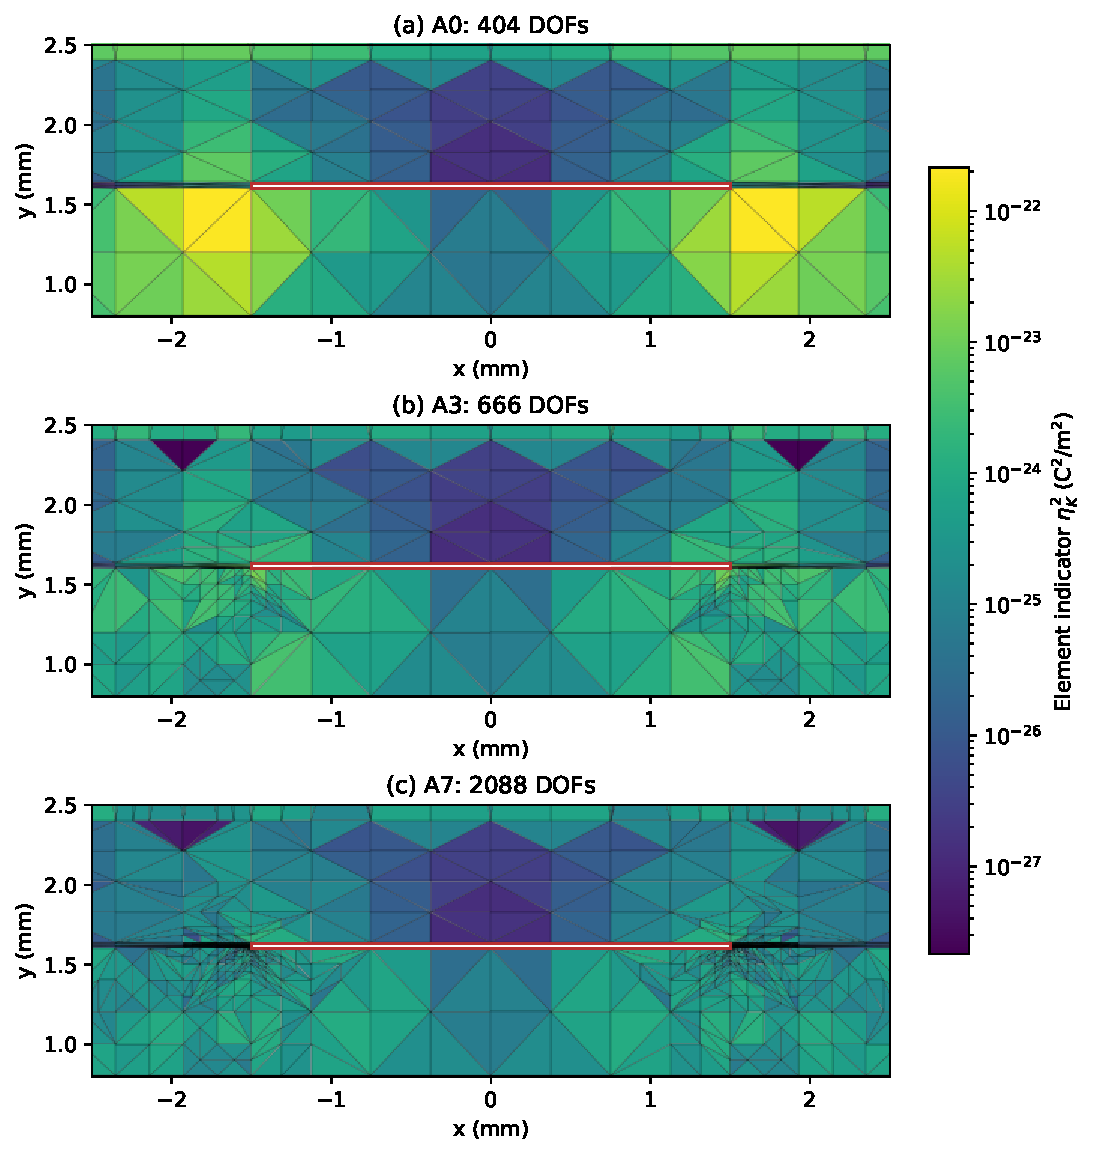
\includegraphics[width=0.88\textwidth,height=0.70\textheight,keepaspectratio]{../figures/adaptive_extension/F_ADAPTIVE_MESH_EVOLUTION.pdf}
\caption{Residual-adaptive meshes A0, A3 and A7 in the same physical near-trace window; colours show $\eta_K^2$ on a shared logarithmic scale. Refinement increasingly concentrates around the trace ends, while some marked regions lie farther into the substrate and air. This is observed localisation, not a claim that the indicator exactly identifies every singular contribution.}
\label{fig:adaptive-mesh}
\end{figure}

Within $0.25H$ of a trace corner, the element fraction rises from $5.11\%$ at A0 to $62.0\%$ at A7; these elements contain $79.6\%$ of the final squared indicator. Initially $88.6\%$ of the indicator is assigned to elements whose nearest corner is a lower junction; at A7 this fraction is $50.2\%$. Thus lower-junction concentration is strongest early, not uniformly dominant throughout. The far-boundary contribution is about $0.00265\%$ of the final indicator. Some final marked element centroids reach $|x|=5.0$ mm and $y=4.57$ mm, so refinement is not confined to four prescribed disks.

\subsection{Matched-work comparison}
One warm-up and five measured repetitions are used for every point. Uniform and graded work includes mesh generation, assembly, solve and capacitance extraction. Adaptive work is cumulative from its initial mesh, including all preceding solves, estimators, marking and refinement, up to the current solution. This accounting deliberately charges adaptive refinement for the preceding solve--estimate--mark--refine cycles because those computations are required to obtain the final adaptive mesh; the comparison is therefore conservative with respect to adaptivity. DOF and NNZ comparisons remain independent of this timing convention. Offline reference solves and error integration are excluded equally. This prevents comparing an entire adaptive trajectory with only a final sparse solve. Millisecond-scale differences on the coarsest meshes are not interpreted as convincing speedups.

\begin{figure}[H]
\centering
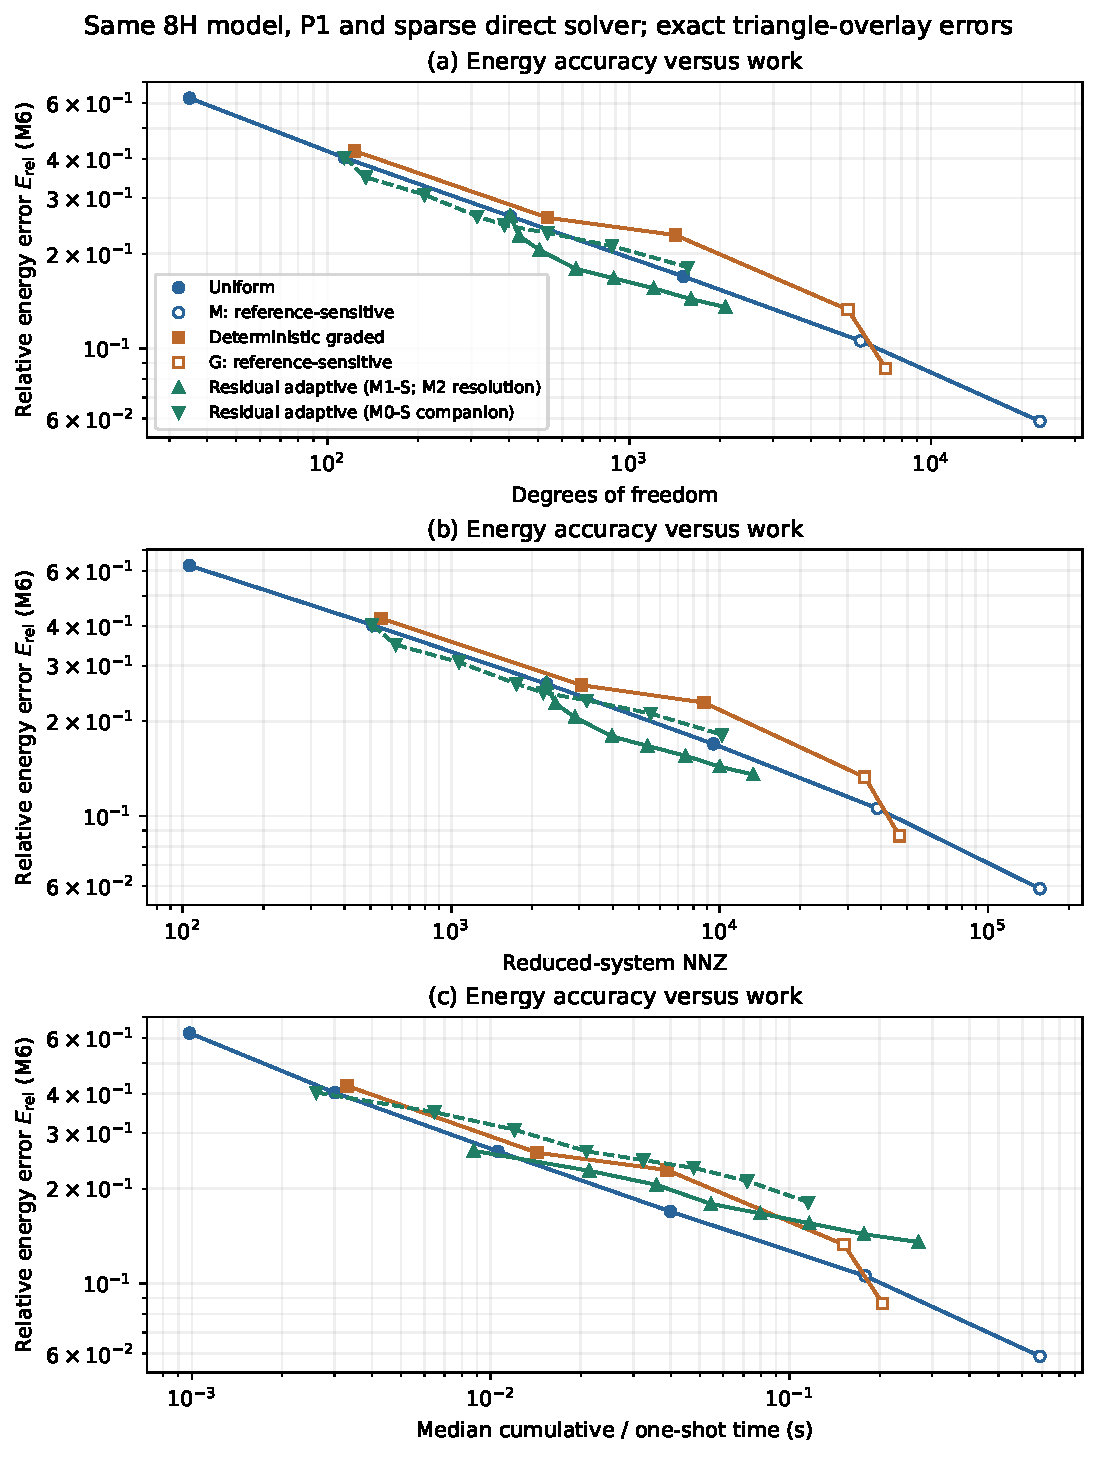
\includegraphics[width=0.92\textwidth,height=0.85\textheight,keepaspectratio]{../figures/adaptive_extension/F_ADAPTIVE_WORK_PRECISION.pdf}
\caption{New three-way comparison in a common norm: (a) DOFs, (b) reduced NNZ, (c) measured median total algorithm time. Solid green triangles are the primary M1-S path; dashed green triangles are its separately identified M0-S companion. Open markers fail the M6/M7 reference-sensitivity threshold. Historical uniform/graded raw errors and timing tables were not overwritten.}
\label{fig:adaptive-work}
\end{figure}

\begin{table}[H]
\centering\small
\caption{Piecewise log-linear interpolation between measured consecutive points only. $U,G,A$ denote uniform, prescribed grading and residual adaptivity. Ratios above one favour adaptivity. The $0.40/0.30$ adaptive targets use the M0-S companion. $^*$The $0.20$ three-way comparison is exploratory because the graded bracket includes reference-sensitive G3.}
\begin{tabular}{@{}lrrrrrr@{}}
\toprule
Target & $N_U$ & $N_G$ & $N_A$ & $N_U/N_A$ & $\mathrm{NNZ}_U/\mathrm{NNZ}_A$ & $T_U/T_A$\\
\midrule
0.40 & 116.6 & 146.2 & 115.1 & 1.013 & 1.022 & 1.115\\
0.30 & 272.8 & 348.7 & 224.0 & 1.218 & 1.235 & 0.546\\
0.20$^*$ & 917.3 & 1974.2 & 532.7 & 1.722 & 1.791 & 0.618\\
\bottomrule
\end{tabular}

\label{tab:adaptive-targets}
\end{table}

At $E_{\rm rel}=0.30$, adaptivity needs about $224$ DOFs versus $273$ for uniform and $349$ for grading, with uniform/adaptive DOF and NNZ ratios $1.218$ and $1.235$. However, its cumulative median time is $13.1$ ms versus $7.15$ ms for uniform: the time ratio is $0.546$, not a speedup. At $0.40$, the DOF ratio is only $1.013$ and the measured times are too small to establish a robust runtime advantage. In a direct reference-stable comparison, A5 uses $1206$ DOFs with error $0.1553$, while M3 uses $1512$ DOFs with error $0.1694$; A5 nevertheless takes about $2.91$ times the cumulative algorithm time.

\subsection{Interpretation and capacitance}
The extension demonstrates an approximation-size advantage at $0.30$, but not a uniform runtime advantage. A7 has $1522$ elements outside the specified corner neighbourhoods, versus $2047$ for G2 at a comparable scale. This supports the explanation that coordinate-line grading spends more resolution away from corners; it does not isolate the causal effects of band width, lower-corner weighting or transitions, which were not varied independently.

The capacitance diagnostic uses $|C_h-C_{M7}|/|C_{M7}|$, where computed M7 is a selected numerical reference, not exact capacitance. A5 differs by $2.42\%$, versus $3.03\%$ for M3, so the energy improvement also has a capacitance benefit in this matched-work pair. A7 still differs by $1.74\%$ and is not substituted for the accepted M7 engineering mesh.

\begin{figure}[H]
\centering
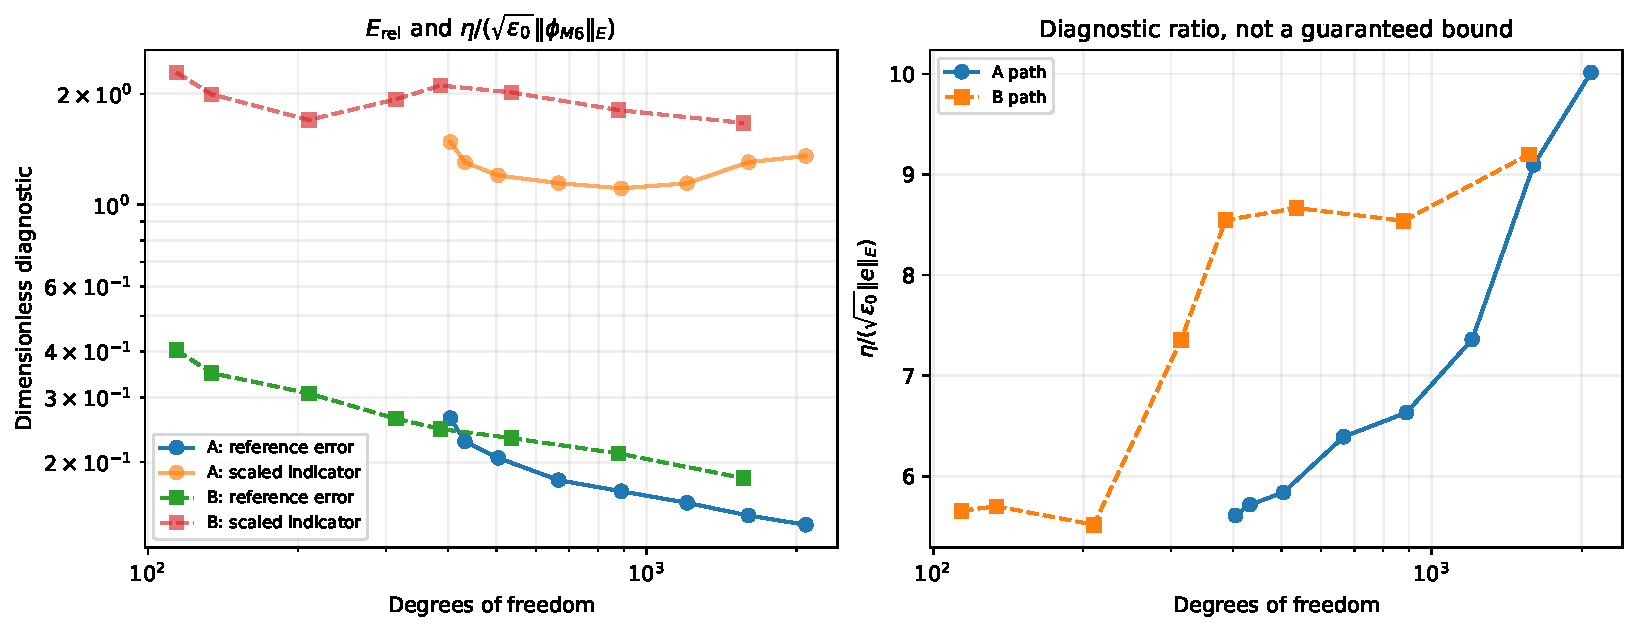
\includegraphics[width=\textwidth]{../figures/adaptive_extension/F_ADAPTIVE_ESTIMATOR.pdf}
\caption{Indicator diagnostics. Physical $\eta$ has units C/m, whereas $\|e\|_E$ has units $\sqrt{\mathrm{J/m}}$. For a dimensionless display only, $\eta$ is divided by $\sqrt{\epsilon_0}$ and the reference norm; the requested unscaled ratio $\eta/\|e\|_E$ is also stored. The dimensionless diagnostic ratio increases from about $5.61$ to $10.0$ on the primary path: it has not stabilised and is not an effectivity constant or guaranteed error bound.}
\label{fig:adaptive-estimator}
\end{figure}

The primary true reference error decreases throughout, but $\eta$ decreases initially and rises again over the last levels. Therefore this indicator is useful for selecting refinement locations in this experiment, but the data do not justify using it as a calibrated stopping criterion. All corrected A/B cycles satisfy potential bounds, symmetry, residual, matrix-symmetry, charge-balance, material and conformity checks; the failed first attempt remains explicitly archived.
